\documentclass{beamer}
\beamerdefaultoverlayspecification{<+->}
%
% Choose how your presentation looks.
%
% For more themes, color themes and font themes, see:
% http://deic.uab.es/~iblanes/beamer_gallery/index_by_theme.html
%
\mode<presentation>
{
  \usetheme{default}      % or try Darmstadt, Madrid, Warsaw, ...
  \usecolortheme{default} % or try albatross, beaver, crane, ...
  \usefonttheme{default}  % or try serif, structurebold, ...
  \setbeamertemplate{navigation symbols}{}
  \setbeamertemplate{caption}[numbered]
  \setbeamertemplate{footline}[frame number]
} 

\usepackage[english]{babel}
\usepackage[utf8]{inputenc}
\usepackage[T1]{fontenc}
\usepackage{hyperref}
\usepackage{pgfplots}
\pgfplotsset{compat=1.7}

\hypersetup{
    colorlinks=true,
    linkcolor=blue,
    filecolor=magenta,      
    urlcolor=cyan,
    bookmarks=true,
    pdfpagemode=FullScreen,
    }

\title{Econ 200 Section AA}
\author{Lukas Hager \newline \href{mailto:lghhager@uw.edu}{lghhager@uw.edu}}
\institute{Office Hours: Wednesday 3-4, Friday 10-11}
\date{October 8, 2021}

\begin{document}

\begin{frame}
  \titlepage
\end{frame}

% Uncomment these lines for an automatically generated outline.
%\begin{frame}{Outline}
%  \tableofcontents
%\end{frame}

\begin{frame}{Your Questions}
    Do you have questions about what you've read in the text or heard in lecture?
\end{frame}

\begin{frame}{Invisible Hand}
    ``\textit{It is not from the benevolence of the butcher, the brewer, or the baker that we expect our dinner, but from their regard to their [self-interest]. . . . he intends only his own gain, and he is in this, as in many other cases, led by an invisible hand to promote an end which was no part of his intention.}" - Adam Smith, Wealth of Nations
\end{frame}

\begin{frame}[t]{Gains from Trade}
    To realize gains from trade, what conditions must be satisfied?
\end{frame}

\begin{frame}[t]{Law of Demand}
   The law of demand says that, when all else is held equal (when all other factors remain the same), quantity demanded rises as price falls.
    \begin{itemize}
        \item All else held equal is sometimes written in Latin as \textit{ceteris paribus}
        \item What is the intuition for why this law is true in general?
        \begin{itemize}
            \item From the textbook: ``What happens when the price of something falls? First, the benefit that you get from purchasing it remains the same because the item itself is unchanged. But the opportunity cost has fallen: When the price goes down, you don’t have to give up as many other purchases in order to get the item. When benefits stay the same and opportunity cost goes down, this trade-off suddenly starts to look a lot better. When the trade-off between costs and benefits tips toward benefits, more people will want to buy the good."
        \end{itemize}
        \item Why is it important to hold everything else equal?
    \end{itemize}
\end{frame}

\begin{frame}{Shifts in Demand}
    \begin{itemize}
        \item What is the difference between an ``increase in demand" and an ``increase in the quantity demanded"?
        \item What non-price factors contribute to demand?
        \begin{itemize}
            \item Income
            \begin{itemize}
                \item Normal goods
                \item Inferior goods
            \end{itemize}
            \item Preferences
            \item Prices of other goods
            \begin{itemize}
                \item Substitutes
                \item Complements
            \end{itemize}
            \item Expectations of future price
            \item Number of consumers
        \end{itemize}
    \end{itemize}
\end{frame}

\begin{frame}{Quantity Demanded vs. Demand}
    Again, from the textbook:
    \begin{itemize}
        \item We say that a change in one of the nonprice determinants of demand causes an ``increase in demand" or ``decrease in demand" -- that is, a shift of the entire demand curve.
        \item To distinguish this from movement along the demand curve, we say that a change in price causes an ``increase in the quantity demanded" or ``decrease in the quantity demanded".
    \end{itemize}
\end{frame}

\begin{frame}{Supply Curves/Shifts in Supply}
    \begin{itemize}
        \item Supply curve shows the \textit{willingness to sell} at each price
        \item Nonprice determinants of supply:
        \begin{itemize}
            \item Prices of related goods
            \item Technology
            \item Prices of inputs
            \item Expectations
            \item Number of sellers
        \end{itemize}
        \item From the textbook: ``Just as with demand, changes in price cause suppliers to move to a different point on the same supply curve, while changes in the nonprice determinants of supply shift the supply curve itself. A change in a nonprice determinant increases or decreases \textit{supply}. A change in price increases or decreases the \textit{quantity supplied}."
    \end{itemize}
\end{frame}

\begin{frame}{Gains from Trade}
    Suppose that France and Germany both produce schnitzel and wine. The following table shows combinations of the goods that each country can produce in a day:
    \begin{table}[]
    \begin{tabular}{|c|c|c|c|}
    \hline
    \multicolumn{2}{|c|}{France}                                                                                              & \multicolumn{2}{c|}{Germany}                                                                                              \\ \hline
    \begin{tabular}[c]{@{}c@{}}Wine \\ (bottles)\end{tabular} & \begin{tabular}[c]{@{}c@{}}Schnitzel \\ (pounds)\end{tabular} & \begin{tabular}[c]{@{}c@{}}Wine \\ (bottles)\end{tabular} & \begin{tabular}[c]{@{}c@{}}Schnitzel \\ (pounds)\end{tabular} \\ \hline
    0                                                         & 8                                                             & 0                                                         & 15                                                            \\ \hline
    1                                                         & 6                                                             & 1                                                         & 12                                                            \\ \hline
    2                                                         & 4                                                             & 2                                                         & 9                                                             \\ \hline
    3                                                         & 2                                                             & 3                                                         & 6                                                             \\ \hline
    4                                                         & 0                                                             & 4                                                         & 3                                                             \\ \hline
                                                              &                                                               & 5                                                         & 0                                                             \\ \hline
    \end{tabular}
    \end{table}
\end{frame}

\begin{frame}{Gains from Trade}
    \begin{table}[]
    \begin{tabular}{|c|c|c|c|}
    \hline
    \multicolumn{2}{|c|}{France}                                                                                              & \multicolumn{2}{c|}{Germany}                                                                                              \\ \hline
    \begin{tabular}[c]{@{}c@{}}Wine \\ (bottles)\end{tabular} & \begin{tabular}[c]{@{}c@{}}Schnitzel \\ (pounds)\end{tabular} & \begin{tabular}[c]{@{}c@{}}Wine \\ (bottles)\end{tabular} & \begin{tabular}[c]{@{}c@{}}Schnitzel \\ (pounds)\end{tabular} \\ \hline
    0                                                         & 8                                                             & 0                                                         & 15                                                            \\ \hline
    1                                                         & 6                                                             & 1                                                         & 12                                                            \\ \hline
    2                                                         & 4                                                             & 2                                                         & 9                                                             \\ \hline
    3                                                         & 2                                                             & 3                                                         & 6                                                             \\ \hline
    4                                                         & 0                                                             & 4                                                         & 3                                                             \\ \hline
                                                              &                                                               & 5                                                         & 0                                                             \\ \hline
    \end{tabular}
    \end{table}
    Who has a comparative advantage in producing wine? In schnitzel?
\end{frame}

\begin{frame}{Gains from Trade}
    \begin{table}[]
    \begin{tabular}{|c|c|c|c|}
    \hline
    \multicolumn{2}{|c|}{France}                                                                                              & \multicolumn{2}{c|}{Germany}                                                                                              \\ \hline
    \begin{tabular}[c]{@{}c@{}}Wine \\ (bottles)\end{tabular} & \begin{tabular}[c]{@{}c@{}}Schnitzel \\ (pounds)\end{tabular} & \begin{tabular}[c]{@{}c@{}}Wine \\ (bottles)\end{tabular} & \begin{tabular}[c]{@{}c@{}}Schnitzel \\ (pounds)\end{tabular} \\ \hline
    0                                                         & 8                                                             & 0                                                         & 15                                                            \\ \hline
    1                                                         & 6                                                             & 1                                                         & 12                                                            \\ \hline
    2                                                         & 4                                                             & 2                                                         & 9                                                             \\ \hline
    3                                                         & 2                                                             & 3                                                         & 6                                                             \\ \hline
    4                                                         & 0                                                             & 4                                                         & 3                                                             \\ \hline
                                                              &                                                               & 5                                                         & 0                                                             \\ \hline
    \end{tabular}
    \end{table}
    Suppose France is currently producing 1 bottle of wine and 6 pounds of schnitzel, and Germany is currently producing 3 bottles of wine and 6 pounds of schnitzel. Demonstrate that France and Germany can both be better off if the specialize in producing only one good and then trade for the other. What are the gains from trade?
\end{frame}

\begin{frame}[t]{Gains from Trade}
    \begin{table}[]
    \begin{tabular}{|c|c|c|c|}
    \hline
    \multicolumn{2}{|c|}{France}                                                                                              & \multicolumn{2}{c|}{Germany}                                                                                              \\ \hline
    \begin{tabular}[c]{@{}c@{}}Wine \\ (bottles)\end{tabular} & \begin{tabular}[c]{@{}c@{}}Schnitzel \\ (pounds)\end{tabular} & \begin{tabular}[c]{@{}c@{}}Wine \\ (bottles)\end{tabular} & \begin{tabular}[c]{@{}c@{}}Schnitzel \\ (pounds)\end{tabular} \\ \hline
    0                                                         & 8                                                             & 0                                                         & 15                                                            \\ \hline
    1                                                         & 6                                                             & 1                                                         & 12                                                            \\ \hline
    2                                                         & 4                                                             & 2                                                         & 9                                                             \\ \hline
    3                                                         & 2                                                             & 3                                                         & 6                                                             \\ \hline
    4                                                         & 0                                                             & 4                                                         & 3                                                             \\ \hline
                                                              &                                                               & 5                                                         & 0                                                             \\ \hline
    \end{tabular}
    \end{table}
\end{frame}

\begin{frame}[t]{Markets}
    Think about a competitive market in which you participate regularly. For each of the characteristics of a competitive market, explain how your market meets these requirements.
\end{frame}

\begin{frame}[t]{Markets}
    Think about a competitive market in which you participate regularly. For each of the characteristics of a competitive market, explain how your market meets these requirements.
    \begin{itemize}
        \item Participants are price-takers
        \item Standardized good
        \item Full information
        \item No transaction costs
    \end{itemize}
\end{frame}

\begin{frame}[t]{Markets}
    Consider shopping for cucumbers in a farmers’ market. For each statement below, note which characteristic of competitive markets the statement describes. Choose from: standardized good, full information, no transaction costs, and participants are price takers.
    \begin{enumerate}
        \item All of the farmers have their prices posted prominently in front of their stalls. 
        \item Cucumbers are the same price at each stall.
        \item There is no difficulty moving around between stalls as you shop and choosing between farmers.
        \item You and the other customers all seem indifferent about which cucumbers to buy.
    \end{enumerate}
\end{frame}

\begin{frame}[t]{Markets}
    Consider shopping for cucumbers in a farmers’ market. For each statement below, note which characteristic of competitive markets the statement describes. Choose from: standardized good, full information, no transaction costs, and participants are price takers.
    \begin{enumerate}
        \item All of the farmers have their prices posted prominently in front of their stalls. (Full information)
        \item Cucumbers are the same price at each stall. (Participants are price takers)
        \item There is no difficulty moving around between stalls as you shop and choosing between farmers. (No transaction costs)
        \item You and the other customers all seem indifferent about which cucumbers to buy. (Standardized good)
    \end{enumerate}
\end{frame}

\begin{frame}[t]{Reading a Demand Curve}
    \begin{table}[]
    \begin{tabular}{|l|l|l|l|l|}
    \hline
    \begin{tabular}[c]{@{}l@{}}Loose Leaf Tea \\ Price \\per lb. \\(dollars)\end{tabular} & \begin{tabular}[c]{@{}l@{}}Sunil's \\Quantity \\Demanded \\ (lbs)\end{tabular} & \begin{tabular}[c]{@{}l@{}}Mia's \\Quantity \\Demanded \\ (lbs)\end{tabular} & \begin{tabular}[c]{@{}l@{}}Rest of \\Market \\Quantity \\Demanded \\ (lbs)\end{tabular} & \begin{tabular}[c]{@{}l@{}}Market \\Quantity \\Demanded \\ (lbs)\end{tabular} \\ \hline
    8                                                                                 & 4                                                                          & 0                                                                        & 30                                                                                &                                                                           \\ \hline
    6                                                                                 & 7                                                                          & 2                                                                        & 40                                                                                &                                                                           \\ \hline
    5                                                                                 & 9                                                                          & 3                                                                        & 51                                                                                &                                                                           \\ \hline
    4                                                                                 & 12                                                                         & 5                                                                        & 64                                                                                &                                                                           \\ \hline
    3                                                                                 & 15                                                                         & 8                                                                        & 90                                                                                &                                                                           \\ \hline
    \end{tabular}
    \end{table}
    The table above shows the demand schedules for loose-leaf tea of two individuals (Sunil and Mia) and the rest of the market. At a price of \$5, the quantity demanded in the market would be?
\end{frame}

\begin{frame}[t]{Reading a Demand Curve}
    \begin{table}[]
    \begin{tabular}{|l|l|l|l|l|}
    \hline
    \begin{tabular}[c]{@{}l@{}}Loose Leaf Tea \\ Price \\per lb. \\(dollars)\end{tabular} & \begin{tabular}[c]{@{}l@{}}Sunil's \\Quantity \\Demanded \\ (lbs)\end{tabular} & \begin{tabular}[c]{@{}l@{}}Mia's \\Quantity \\Demanded \\ (lbs)\end{tabular} & \begin{tabular}[c]{@{}l@{}}Rest of \\Market \\Quantity \\Demanded \\ (lbs)\end{tabular} & \begin{tabular}[c]{@{}l@{}}Market \\Quantity \\Demanded \\ (lbs)\end{tabular} \\ \hline
    8                                                                                 & 4                                                                          & 0                                                                        & 30                                                                                &                                                                           \\ \hline
    6                                                                                 & 7                                                                          & 2                                                                        & 40                                                                                &                                                                           \\ \hline
    5                                                                                 & 9                                                                          & 3                                                                        & 51                                                                                &                                                                           \\ \hline
    4                                                                                 & 12                                                                         & 5                                                                        & 64                                                                                &                                                                           \\ \hline
    3                                                                                 & 15                                                                         & 8                                                                        & 90                                                                                &                                                                           \\ \hline
    \end{tabular}
    \end{table}
    The table above shows the demand schedules for loose-leaf tea of two individuals (Sunil and Mia) and the rest of the market. If the price of loose-leaf tea rises from \$3 to \$4, the market quantity demanded would?
\end{frame}

\begin{frame}[t]{Demand/Supply Curves}
    Graph the equation $P = -8Q + 10$. Is this the supply curve or demand curve?
\end{frame}

\begin{frame}[t]{Demand/Supply Curves}
    Graph the equation $P = -8Q + 10$. Is this the supply curve or demand curve?
    \begin{tikzpicture}
    \begin{axis}[
        axis lines = left,
        xmin=0, xmax=2,
        ymin=0, ymax=12,
        xlabel = {$Q$},
        ylabel = {$P$},
    ]
    \addplot[thick] {-8*x + 10};
    \end{axis}
    \end{tikzpicture}
\end{frame}

\begin{frame}[t]{Demand/Supply Curves}
    Rearrange the equation $Q = 5 - 0.25P$ and sketch the graph. Is this a supply curve or a demand curve?
\end{frame}

\begin{frame}[t]{Demand/Supply Curves}
    Rearrange the equation $Q = 5 - 0.25P$ and sketch the graph. Is this a supply curve or a demand curve?
    \[\begin{split}
        &Q = 5 - 0.25P \\
        \implies &Q-5 = -0.25P \\
        \implies &\frac{Q-5}{-0.25} = P \\
        \implies &\boxed{P = -4Q + 20}
    \end{split}\]
\end{frame}

\begin{frame}[t]{Demand/Supply Curves}
    Rearrange the equation $Q = 5 - 0.25P$ and sketch the graph. Is this a supply curve or a demand curve?
    \begin{tikzpicture}
    \begin{axis}[
        axis lines = left,
        xmin=0, xmax=6,
        ymin=0, ymax=25,
        xlabel = {$Q$},
        ylabel = {$P$},
    ]
    \addplot[thick] {-4*x + 20};
    \end{axis}
    \end{tikzpicture}
\end{frame}

\begin{frame}{Demand for iPhones}
    Apple raises the price of iPhones.
    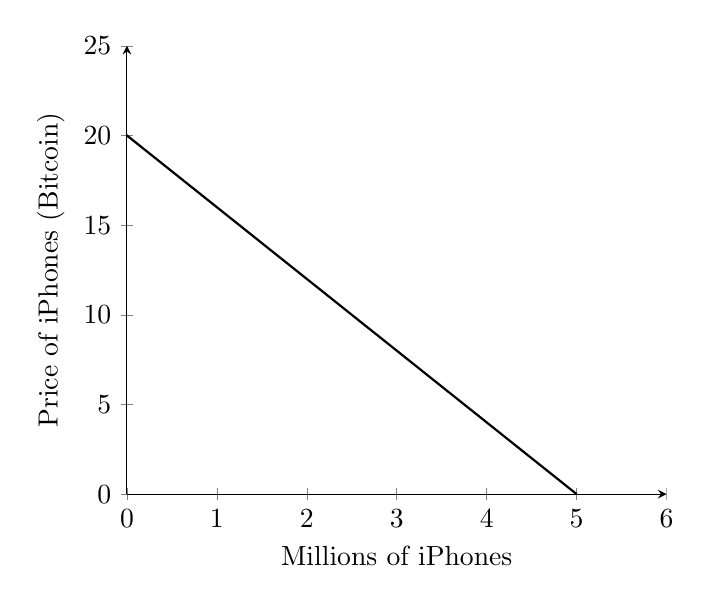
\begin{tikzpicture}
    \begin{axis}[
        axis lines = left,
        xmin=0, xmax=6,
        ymin=0, ymax=25,
        xlabel = {Millions of iPhones},
        ylabel = {Price of iPhones (Bitcoin)},
    ]
    \addplot[thick] {-4*x + 20};
    \end{axis}
    \end{tikzpicture}
\end{frame}

\begin{frame}{Demand for iPhones}
    Samsung raises the price of the Galaxy.
    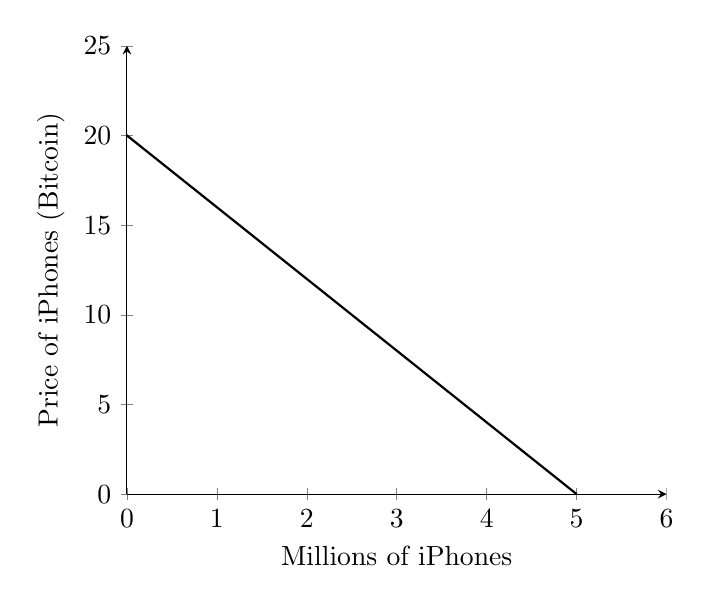
\begin{tikzpicture}
    \begin{axis}[
        axis lines = left,
        xmin=0, xmax=6,
        ymin=0, ymax=25,
        xlabel = {Millions of iPhones},
        ylabel = {Price of iPhones (Bitcoin)},
    ]
    \addplot[thick] {-4*x + 20};
    \end{axis}
    \end{tikzpicture}
\end{frame}

\begin{frame}{Demand for iPhones}
    The cost of iPhone apps goes up.
    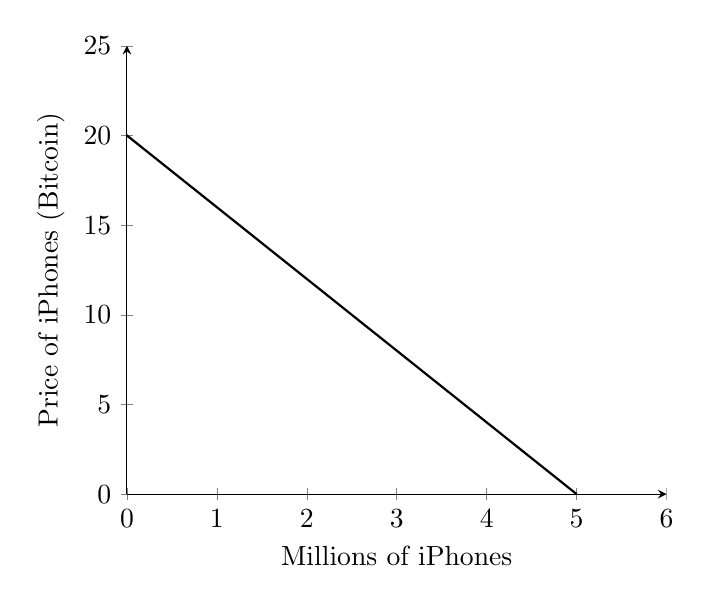
\begin{tikzpicture}
    \begin{axis}[
        axis lines = left,
        xmin=0, xmax=6,
        ymin=0, ymax=25,
        xlabel = {Millions of iPhones},
        ylabel = {Price of iPhones (Bitcoin)},
    ]
    \addplot[thick] {-4*x + 20};
    \end{axis}
    \end{tikzpicture}
\end{frame}

\begin{frame}{Demand for iPhones}
    New research shows that iPhones cause finger cancer.
    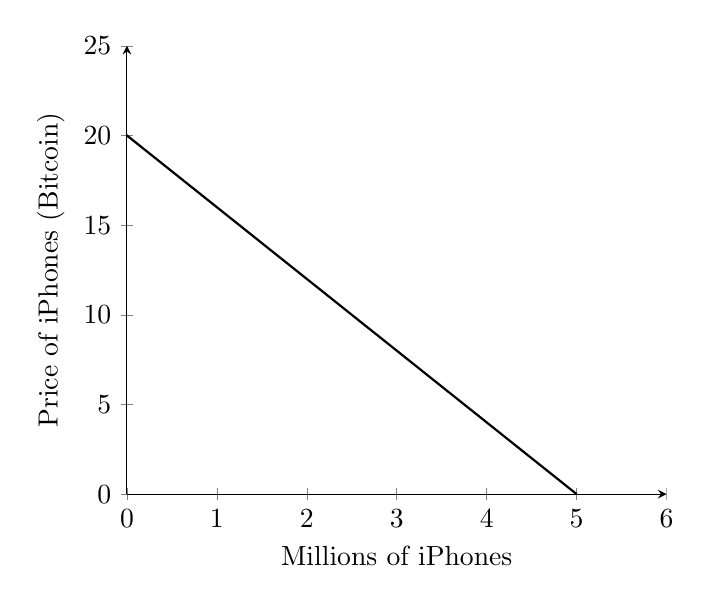
\begin{tikzpicture}
    \begin{axis}[
        axis lines = left,
        xmin=0, xmax=6,
        ymin=0, ymax=25,
        xlabel = {Millions of iPhones},
        ylabel = {Price of iPhones (Bitcoin)},
    ]
    \addplot[thick] {-4*x + 20};
    \end{axis}
    \end{tikzpicture}
\end{frame}

\begin{frame}{Demand for iPhones}
    A recession hits and incomes fall.
    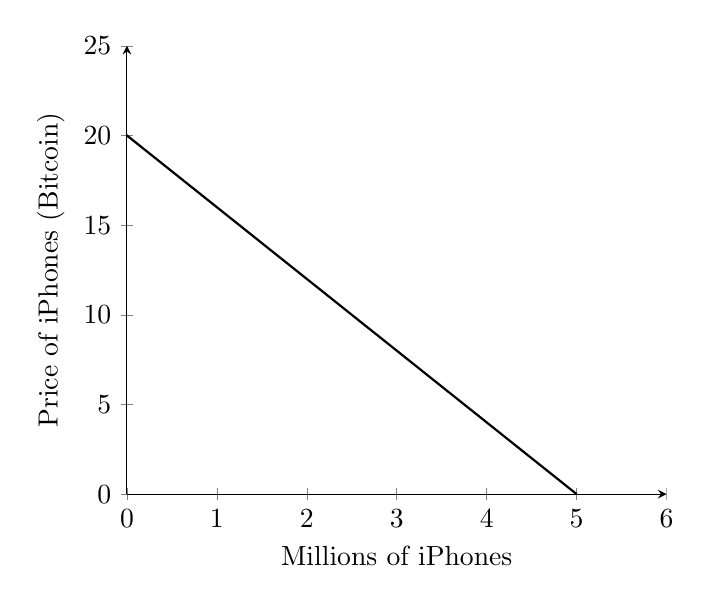
\begin{tikzpicture}
    \begin{axis}[
        axis lines = left,
        xmin=0, xmax=6,
        ymin=0, ymax=25,
        xlabel = {Millions of iPhones},
        ylabel = {Price of iPhones (Bitcoin)},
    ]
    \addplot[thick] {-4*x + 20};
    \end{axis}
    \end{tikzpicture}
\end{frame}

\begin{frame}{Ceteris Paribus}
    Why is including the phrase \textit{ceteris paribus} important when we discuss moving along the demand curve?
\end{frame}

\begin{frame}[t]{Supply Shifts}
    \begin{tikzpicture}
    \begin{axis}[
        axis lines = left,
        xmin=0, xmax=6,
        ymin=0, ymax=25,
        xlabel = {$Q$},
        ylabel = {$P$},
    ]
    \addplot[thick] {4*x};
    \addplot[thick] {4*x + 5};
    \node[label={0:{A}},circle,fill,inner sep=2pt] at (axis cs:2, 13) {};
    \node[label={0:{B}},circle,fill,inner sep=2pt] at (axis cs:4, 21) {};
    \node[label={0:{C}},circle,fill,inner sep=2pt] at (axis cs:3, 12) {};
    \end{axis}
    \end{tikzpicture} \\
    What are some factors that would move suppliers from point A to point B?
\end{frame}

\begin{frame}[t]{Supply Shifts}
    \begin{tikzpicture}
    \begin{axis}[
        axis lines = left,
        xmin=0, xmax=6,
        ymin=0, ymax=25,
        xlabel = {$Q$},
        ylabel = {$P$},
    ]
    \addplot[thick] {4*x};
    \addplot[thick] {4*x + 5};
    \node[label={0:{A}},circle,fill,inner sep=2pt] at (axis cs:2, 13) {};
    \node[label={0:{B}},circle,fill,inner sep=2pt] at (axis cs:4, 21) {};
    \node[label={0:{C}},circle,fill,inner sep=2pt] at (axis cs:3, 12) {};
    \end{axis}
    \end{tikzpicture} \\
    What are some factors that would move suppliers from point A to point C? C to B?
\end{frame}

\begin{frame}[t]{Finding Equilibrium}
    The demand and supply equations for the market for oil changes in Seattle are:
    \begin{itemize}
        \item Demand: $Q=12000 - 100P$
        \item Supply: $Q=50P$
        \item $P$ = price per oil change, and $Q$ = quantity of oil changes per day
    \end{itemize}
    Calculate the equilibrium price and quantity.
\end{frame}

\begin{frame}[t]{Finding Equilibrium}
    The demand and supply equations for the market for oil changes in Seattle are:
    \begin{itemize}
        \item Demand: $Q=12000 - 100P$
        \item Supply: $Q=50P$
        \item $P$ = price per oil change, and $Q$ = quantity of oil changes per day
    \end{itemize}
    Draw the supply and demand curves on the graph below. Be sure to label the y-intercepts of each graph and the equilibrium. Label the supply curve $S$ and the demand curve $D$.
\end{frame}

\begin{frame}[t]{Finding Equilibrium}
    Draw the supply and demand curves on the graph below. Be sure to label the y-intercepts of each graph and the equilibrium. Label the supply curve $S$ and the demand curve $D$.
\end{frame}

\end{document}
